% ==============================================================================
% SECCIÓN DE INTEGRACIÓN Y PROTOTIPO INTERACTIVO (FORMATO IEEEtran)
% ==============================================================================

\section{Integraci\'on de Software, Visualizaci\'on y Prototipo Interactivo}
\label{sec:integration}

\subsection{Puente End-to-End sin Intervenci\'on Manual}
El sistema articula la fase sensorial y el motor de programaci\'on por restricciones de manera completamente autom\'atica a trav\'es de la funci\'on principal \texttt{solve\_image(image\_path, method="auto")}:

\begin{enumerate}
    \item La imagen es procesada por el pipeline de visi\'on, extrayendo la geometr\'{\i}a de la grilla, las celdas de cada jaula y la lista ordenada de candidatos OCR $(T_{c,k}, \text{op}_{c,k}, P_{c,k})$.
    \item Se instancia una resoluci\'on r\'apida con la \textbf{Variante A (Aritm\'etica Intensional)} utilizando las lecturas Top-1.
    \item Si el solver reporta \texttt{OPTIMAL}, la soluci\'on es retornada en menos de $0.28\text{ s}$ en promedio.
    \item Si las lecturas Top-1 contienen alguna inconsistencia sensorial que torne el modelo en \texttt{INFEASIBLE}, el lazo de integraci\'on conmuta autom\'aticamente y sin intervenci\'on humana a la \textbf{Variante C (Inferencia Conjunta MAP)}, resolviendo las ambig\"uedades bajo regularizaci\'on $\ell_0$.
\end{enumerate}

El repositorio completo del proyecto est\'a alojado en GitHub: \url{https://github.com/JoanixX/kenken-vision-cp-solver}.

\subsection{Motor de Renderizado y Proyecci\'on Visual}
Para garantizar una comprensi\'on visual inmediata de la soluci\'on, el sistema provee cuatro modalidades gr\'aficas de salida:
\begin{enumerate}
    \item \textbf{Modo \texttt{original}:} Proyecta los n\'umeros resueltos directamente sobre la fotograf\'{\i}a original, deformando las fuentes y coordenadas espaciales mediante la transformaci\'on homogr\'afica proyectiva inversa $H^{-1}$.
    \item \textbf{Modo \texttt{composite}:} Genera una infograf\'{\i}a de resoluci\'on comparativa que exhibe la imagen de entrada junto a la cuadr\'{\i}cula vectorial resuelta (Fig.~\ref{fig:e2e_demo}).
    \item \textbf{Modo \texttt{clean}:} Genera una cuadr\'{\i}cula gr\'afica vectorial n\'{\i}tida en alta resoluci\'on, apta para impresi\'on o publicaci\'on.
    \item \textbf{Modo \texttt{rectified}:} Superpone los valores calculados sobre el plano frontal rectificado tras la correcci\'on de perspectiva.
\end{enumerate}

\begin{figure}[htbp]
\centering
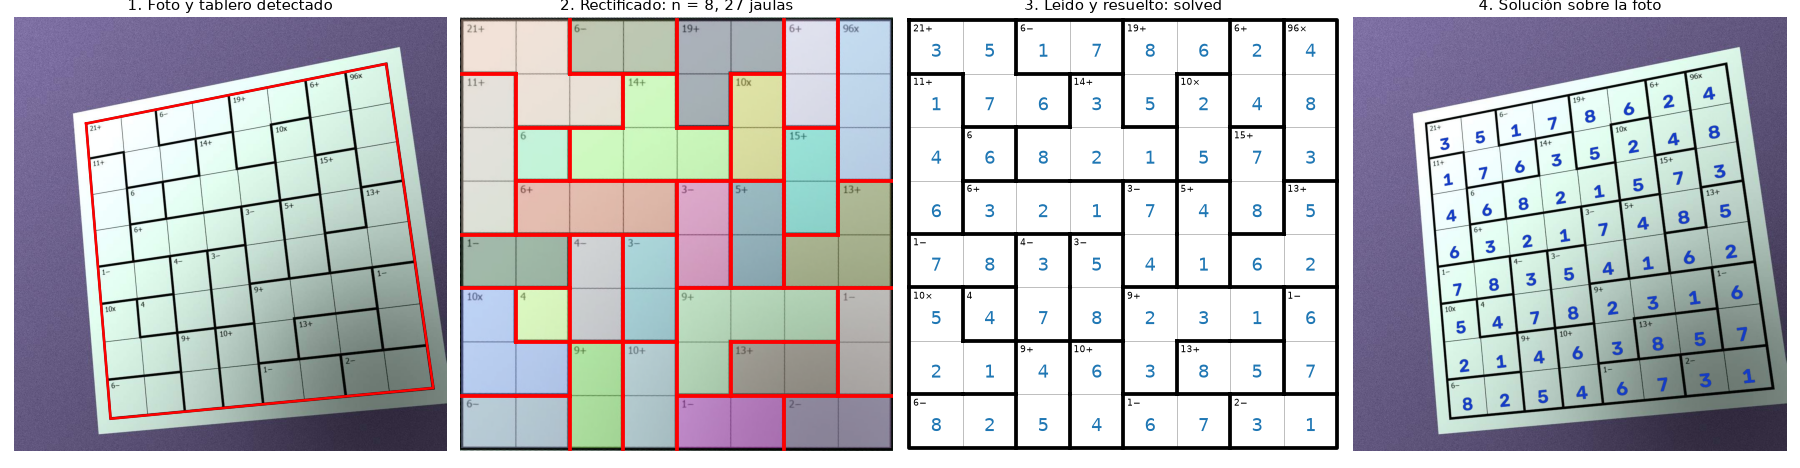
\includegraphics[width=\linewidth]{figs/e2e_photo_8x8.png}
\caption{Demostraci\'on de resoluci\'on End-to-End sobre una fotograf\'{\i}a real de KenKen $8 \times 8$: integraci\'on continua desde la captura inclinada hasta la visualizaci\'on infogr\'afica con superposici\'on de resultados.}
\label{fig:e2e_demo}
\end{figure}

\subsection{Prototipo Interactivo Desplegado en la Nube (Hugging Face Spaces)}
Para permitir la experimentaci\'on interactiva y auditor\'{\i}a en tiempo real por parte de la comunidad acad\'emica y evaluadores, el sistema fue empaquetado y desplegado como una aplicaci\'on web p\'ublica en la plataforma \textbf{Hugging Face Spaces} utilizando Gradio, accesible en vivo en \url{https://huggingface.co/spaces/joako2202/kenken-solver}.

La aplicaci\'on en la nube incorpora:
\begin{itemize}
    \item \textbf{Carga y Diagn\'ostico en Vivo:} Admite arrastrar y soltar cualquier imagen, desplegando en tiempo real el tiempo de ejecuci\'on, el estado del solver y el informe del sem\'aforo de fiabilidad.
    \item \textbf{Panel de Transparencia Neuro-Simb\'olica:} Si la inferencia conjunta MAP se activa, la interfaz detalla con vi\~netas legibles cu\'ales jaulas fueron ajustadas (e.g., \textit{Jaula 2: Top-1 visual '4/' $\to$ Corregido a '2/'}), la m\'etrica de fidelidad visual porcentual y el nivel cualitativo de confianza (\texttt{HIGH}, \texttt{MODERATE}, \texttt{LOW}).
    \item \textbf{Cat\'alogo Demostrativo de 21 Muestras:} Incorpora 3 instancias seleccionadas para cada uno de los 7 perfiles operacionales del sistema: (1) Lectura directa, (2) Rescate MAP, (3) Perspectiva y rotaci\'on, (4) Gran escala hasta $9\times9$, (5) Rescate de estr\'es, (6) Aviso de verificaci\'on por m\'ultiples ajustes, y (7) Detecci\'on de infactibilidad honesta.
\end{itemize}
